%%%%%%%%%%%%%%%%%%%%%%%%%%%
%
% $Autor: Vikas Ramaswamy$
% $Datum: 2023-03-17 11:15:45Z $
% $Pfad: GDV/Vortraege/latex - Ausarbeitung/Kapitel/MapleDateien.tex $
% $Version: 4732 $
%
%%%%%%%%%%%%%%%%%%%%%%%%%%%
%\VERSION{$ $Pfad: GDV/Vortraege/latex - Ausarbeitung/Kapitel/MapleDateien.tex $ $}{$ $Version: 4732 $ $}



\chapter{Data Mining - Algorithms for Pneumonia detection}


\section{Random Forest}

Random Forest is an ensemble learning algorithm that combines multiple decision trees to make predictions. It creates a set of decision trees on randomly selected data samples, and the final prediction is made by aggregating the predictions of individual trees. Each tree in the forest independently makes a prediction, and the final result is determined by majority voting or averaging the predictions. \autocite{Breiman:2001}

\subsection{Applications:}

Random Forest has a large area of application. However, some of the applications are:\\

\begin{enumerate}

\item \textbf{Pneumonia detection:} Random Forest can be used to classify chest X-ray images as pneumonia or non-pneumonia cases.
\item \textbf{Medical diagnosis}: It can assist in diagnosing various medical conditions by analyzing relevant features.
\item \textbf{Image classification:} Random Forest can be employed for classifying images into different categories based on their features.

\end{enumerate}

\subsection{Relevance:}

Random Forest is particularly suitable for pneumonia detection due to its ability to handle high-dimensional data, provide feature importance ranking, and effectively handle imbalanced datasets. It can handle both classification and regression tasks and is robust against overfitting.\\


\subsection{Hyperparameters:}

\begin{enumerate}
\item \textbf{Number of trees:} The number of decision trees to be created in the random forest.\\
\item \textbf{Maximum depth:}The maximum depth allowed for each decision tree in the forest.\\
\item \textbf{Minimum samples split:} The minimum number of samples required to split a node further.\\
\item \textbf{Maximum features:} The number of features to consider when looking for the best split.\\
\end{enumerate}

\subsection{Requirements:}
\begin{enumerate}
\item \textbf{Labeled training data:} A dataset with chest X-ray images and corresponding labels indicating whether the image represents a pneumonia case or not.\\
\item \textbf{Preprocessing:} The input data should be preprocessed, including image resizing, normalization, and feature extraction.\\
\end{enumerate}

\subsection{Input:}
Training data consists of chest X-ray images, represented as feature vectors, along with their corresponding labels indicating pneumonia or non-pneumonia cases.\\

\subsection{Output:}
The Random Forest algorithm outputs predicted class labels for unseen chest X-ray images, indicating whether they are classified as pneumonia or non-pneumonia cases.\\


\section{Support Vector Machines (SVM)}

\ac{SVM} is a supervised machine learning technique that is used for classification and regression applications. SVM separates data points by locating the best hyperplane in a multidimensional feature space. It can handle both linear and non-linear data and seeks to optimize the margin between classes.\autocite{cortes:2009}


\subsection{Relevance:}

SVM is particularly relevant for pneumonia detection as it can handle complex datasets, especially those with clear margin separation. It is effective in dealing with high-dimensional data and can provide accurate predictions when properly tuned.\\


\subsection{Hyperparameters:}

\begin{enumerate}
	\item \textbf{Kernel type:}  SVM supports various kernel functions (e.g., linear, polynomial, radial basis function) that transform the data to a higher-dimensional space.\\
	\item \textbf{Regularization parameter (C):} It controls the trade-off between maximizing the margin and minimizing the classification errors.\\
	\item \textbf{Gamma parameter:}  It determines the influence of each training example on the decision boundary for non-linear kernels.\\
\end{enumerate}

\subsection{Requirements:}
\begin{enumerate}
	\item \textbf{Labeled training data:} A dataset with chest X-ray images and corresponding labels indicating whether the image represents a pneumonia case or not.\\
	\item \textbf{Preprocessing:} The input data should be preprocessed, including image resizing, normalization, and feature extraction.\\
\end{enumerate}

\subsection{Input:}
Training data consists of chest X-ray images, represented as feature vectors, along with their corresponding labels indicating pneumonia or non-pneumonia cases.\\

\subsection{Output:}
The SVM algorithm outputs predicted class labels for unseen chest X-ray images, indicating whether they are classified as pneumonia or non-pneumonia cases.\\


\section{Convolutional Neural Networks}

Deep learning methods known as \ac{cnn}) are extensively utilized for image classification applications. CNNs are made up of numerous convolutional and pooling layers, followed by fully linked classification layers. They are intended to learn hierarchical representations from incoming photos automatically.\autocite{lecun:1998}

\subsection{Relevance:}

CNNs are useful for detecting pneumonia because they excel at learning spatial hierarchies of data from images. They can detect complicated patterns and relationships in medical imagery, allowing them to accurately diagnose pneumonia.\\


\subsection{Hyperparameters:}

\begin{enumerate}
	\item \textbf{Number and size of filters: } CNNs use filters for feature extraction. The number and size of filters determine the complexity and depth of the network.\\
	\item \textbf{Learning rate:} It controls the step size during the gradient descent optimization process.\\
	\item \textbf{Dropout rate:} Dropout is a regularization technique used to prevent overfitting. The dropout rate specifies the probability of randomly dropping out nodes during training.\\
	\item \textbf{Batch size:} The number of training examples used in each iteration of training.\\
\end{enumerate}


\subsection{Requirements:}
\begin{enumerate}
	\item \textbf{Labeled training data:} A dataset with chest X-ray images and corresponding labels indicating whether the image represents a pneumonia case or not.\\
	\item \textbf{Computational resources:} Training CNNs can be computationally intensive, so access to GPUs or other high-performance hardware is beneficial.\\
\end{enumerate}

\subsection{Input:}
Images of chest X-rays, typically in the form of 2D arrays or tensors.\\

\subsection{Output:}
The CNN algorithm outputs predicted class labels for unseen chest X-ray images, indicating whether they are classified as pneumonia or non-pneumonia cases.\\

\section{Examples for the Algorithms}

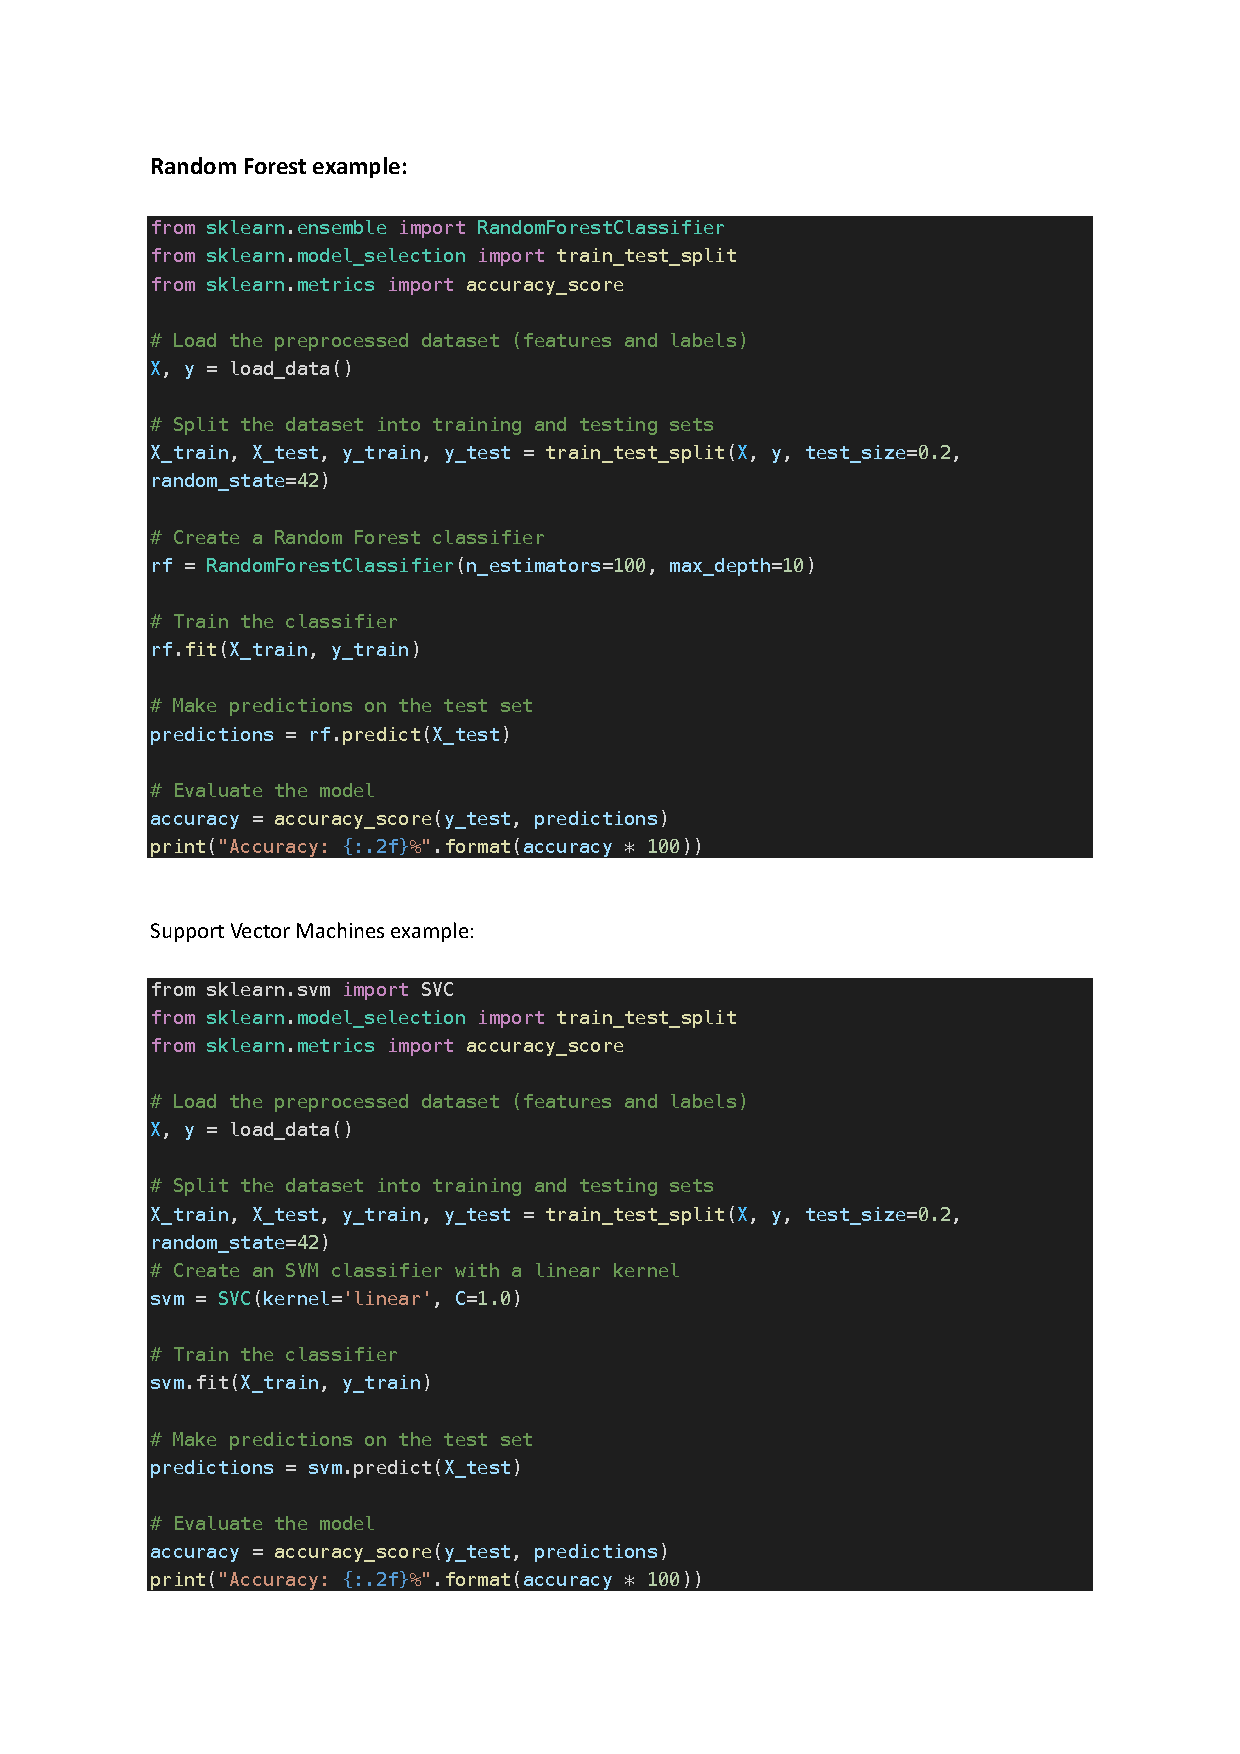
\includepdf[pages={-}]{Code/AlgorithmExamples.pdf}
